\documentclass{article}
\usepackage{amsmath,amssymb,graphicx,hyperref,geometry,listings,booktabs}
\usepackage{xcolor}
\usepackage{longtable}
\usepackage{tikz}
\usepackage{pgfplots}
\usepackage{array}
\usetikzlibrary{arrows.meta,positioning,fit,backgrounds}
\pgfplotsset{compat=1.18}
\newcolumntype{P}[1]{>{\raggedright\arraybackslash}p{#1}}

\geometry{margin=1in}
\hypersetup{
    colorlinks=true,
    linkcolor=blue,
    citecolor=blue,
    urlcolor=blue
}

\lstdefinestyle{paperstyle}{
    basicstyle=\ttfamily\small,
    keywordstyle=\color{blue!70!black},
    commentstyle=\color{green!40!black},
    stringstyle=\color{red!60!black},
    numbers=left,
    numberstyle=\tiny\color{gray},
    stepnumber=1,
    numbersep=8pt,
    showstringspaces=false,
    breaklines=true,
    frame=single,
    tabsize=2
}
\lstset{style=paperstyle}

\title{\textbf{HypeStock: A Production AI Stock Forecasting System with Telemetry-Grounded Optimization and Compressed Conversation Memory}}
\author{DAP391 Research Engineering Group}
\date{March 2026}

\begin{document}

\maketitle

\begin{abstract}
This paper presents a production-grade stock forecasting platform that unifies a high-throughput machine learning stack with a latency-critical online serving architecture. The deployed system combines FastAPI plus Socket.IO, PostgreSQL plus TimescaleDB, Celery, Redis, and Nginx with a hybrid forecasting backbone composed of a Transformer encoder, attention pooling, GRU decoder, and LightGBM residual ensembling. The AI layer integrates Gemini and PandasAI for grounded natural-language interaction.

A new architecture component is introduced: a self-implemented SessionMemory module is integrated as a compressed cross-message memory subsystem that stores and retrieves semantically compressed client and backend interactions. This enables continuity in AI responses without unbounded prompt growth.

Although the model architecture supports multi-horizon outputs (7, 14, and 30 days), deployment is intentionally specialized to the 7-day horizon. We provide formal loss derivations, gradient interference analysis, and empirical validation from real training telemetry. We further analyze runtime parameters, optimization stability, and hardware-aware throughput behavior on Ryzen 7 7435HS plus RTX 4060 Laptop (16 GB RAM), using observed metrics including \texttt{pred\_mean}, \texttt{pred\_std}, \texttt{volatility\_loss}, \texttt{curvature\_loss}, and \texttt{acf1}.
\end{abstract}

\tableofcontents
\newpage

\section{Introduction}
Production forecasting systems fail when model design, data systems, and runtime infrastructure are optimized in isolation. In equity prediction, this mismatch appears as unstable calibration, stale context, queue backpressure, and brittle explanation quality under changing market regimes. HypeStock is designed as an end-to-end system where database shape, model objective, queueing policy, and user-facing AI behavior are co-optimized.

The central engineering decision in this paper is a controlled collapse from multi-horizon capability to single-horizon deployment, while preserving extensibility in the model interface and data schema. The central architecture decision is to add a self-implemented compressed memory component that captures all client and backend messages in semantically compressed form.

\section{System Architecture and New Memory Component}
\subsection{Service Topology}
The production topology includes:
\begin{itemize}
\item FastAPI plus Socket.IO as the API and streaming plane.
\item PostgreSQL plus TimescaleDB for historical and derived time-series storage.
\item Celery for asynchronous model and analytics jobs.
\item Redis for broker plus cache roles.
\item Nginx for reverse proxying and static frontend delivery.
\item PyTorch plus LightGBM for prediction.
\item Gemini plus PandasAI for explanation and structured AI query handling.
\end{itemize}

End-to-end latency can be decomposed as
\begin{equation}
T_{e2e}=T_{fetch}+T_{feature}+T_{predict}+T_{cache}+T_{transport}.
\end{equation}

\begin{figure}[t]
\centering
\begin{tikzpicture}[
    >=Latex,
    node distance=2.00cm and 1.90cm,
    svc/.style={draw, rounded corners, thick, minimum width=3.2cm, minimum height=1.0cm, align=center, fill=white, font=\small},
    tinyann/.style={font=\scriptsize, text=black!75, align=center},
    grp/.style={draw=black!55, rounded corners, thick, inner sep=10pt}
]
\node[svc] (client) {Web client};
\node[svc, right=of client] (nginx) {Nginx\\reverse proxy};
\node[svc, right=of nginx] (api) {FastAPI +\\Socket.IO};

\node[svc, below=3.30cm of client] (gemini) {Gemini + PandasAI};
\node[svc, right=of gemini] (memory) {SessionMemory\\(compressed history)};
\node[svc, right=of memory, minimum width=6.2cm, text width=4.5cm] (model) {Transformer + Attention + GRU\\+ LightGBM residual};

\node[svc, below=3.40cm of gemini] (redis) {Redis\\broker + cache};
\node[svc, right=of redis] (celery) {Celery workers};
\node[svc, right=of celery] (tsdb) {PostgreSQL +\\TimescaleDB};

\draw[->, thick] (client) -- (nginx);
\draw[->, thick] (nginx) -- (api);

\draw[<->, thick] (api.south) -- ++(0,-1.55cm) -| (gemini.north);
\draw[<->, thick] (gemini) -- (memory);
\draw[<->, thick] (memory) -- (model);

\draw[->, thick] (api.east) -- ++(4.05cm,0) |- (celery.east);
\draw[<->, thick] (api.east) -- ++(4.05cm,0) |- (tsdb.east);
\draw[<->, thick] (api.west) -- ++(-1.35cm,0) |-Z (redis.west);
\draw[<->, thick] (celery) -- (redis);
\draw[<->, thick] (celery) -- (tsdb);
\draw[->, thick] (tsdb.north) -- ++(0,1.20cm) -| (model.south);

\begin{scope}[on background layer] 
\node[grp, fill=blue!4, fit=(client) (nginx) (api), label={[font=\footnotesize,yshift=3pt]above:Serving plane}] (servinggrp) {};
\node[grp, fill=green!4, fit=(gemini) (memory) (model), label={[font=\footnotesize,yshift=3pt,xshift=-24pt]above:AI and model plane}] (aigrp) {};
\node[grp, fill=orange!6, fit=(redis) (celery) (tsdb), label={[font=\footnotesize,yshift=3pt]above:Async and data plane}] (asyncgrp) {};
\end{scope}

\node[tinyann, anchor=south] at ([xshift=-1.2cm,yshift=1.45cm]aigrp.north) {all client/backend messages\\semantically compressed};
\node[tinyann, anchor=north] at ([yshift=-1.45cm]asyncgrp.south) {async retraining, backfill,\\feature jobs};
\node[tinyann, anchor=south] at ([xshift=-5.25cm,yshift=-1.8cm]aigrp.east) {7-day horizon\\online inference};
\end{tikzpicture}
\caption{End-to-end production architecture with the new self-implemented SessionMemory component.}
\label{fig:architecture}
\end{figure}

\subsection{Self-Implemented SessionMemory Component for Compressed Client and Backend Messages}
The new component uses HypeStock's self-implemented SessionMemory module as a session-scoped compression and retrieval subsystem. For each websocket session $s$, the complete interaction stream is
\begin{equation}
M^{(s)}=\{(r_i,c_i,t_i)\}_{i=1}^{N_s}, \quad r_i \in \{\text{client},\text{backend}\},
\end{equation}
where $c_i$ is message content and $t_i$ is timestamp.

SessionMemory applies semantic compression
\begin{equation}
Z^{(s)}=\mathcal{C}_{HS}(M^{(s)}),
\end{equation}
and query-aware retrieval
\begin{equation}
H_q^{(s)}=\mathcal{R}_{HS}(q,Z^{(s)},k),
\end{equation}
with $k$ bounded summary bullets injected into the classifier and response prompts.

This design removes the previous fixed-length truncation and replaces it with compressed history over all recorded client and backend interactions in the session.

\section{Forecasting Model Formulation}
\subsection{Sliding Window Construction}
Given a lookback $L$, each training sample is formed by
\begin{equation}
X_t=[x_{t-L},\ldots,x_t],
\end{equation}
where $x_t \in \mathbb{R}^d$ is the multivariate feature vector at time $t$.

\subsection{Transformer Encoder}
The attention block follows
\begin{equation}
\text{Attention}(Q,K,V)=\text{softmax}\left(\frac{QK^T}{\sqrt{d_k}}\right)V.
\end{equation}

This supports long-range feature interactions across volatility, momentum, and microstructure channels before temporal decoding.

\subsection{GRU Decoder Dynamics}
The recurrent decoder is governed by
\begin{equation}
z_t = \sigma(W_z x_t + U_z h_{t-1}),
\end{equation}
\begin{equation}
r_t = \sigma(W_r x_t + U_r h_{t-1}),
\end{equation}
\begin{equation}
h_t = (1 - z_t) \odot h_{t-1} + z_t \odot \tilde{h}_t.
\end{equation}

The deployed output map is
\begin{equation}
\hat{y}_{t+7}=f(x_{t-L:t}).
\end{equation}

\section{Multi-Horizon Objective and 7-Day Collapse}
\subsection{General Objective}
Architecture-level training supports a horizon set $H=\{7,14,30\}$ with weighted objective
\begin{equation}
\mathcal{L}_{multi} = \sum_{h \in H} \alpha_h \cdot \mathcal{L}_h.
\end{equation}

Deployment is specialized to
\begin{equation}
\mathcal{L}_{7} = \mathcal{L}_{h=7}.
\end{equation}

\subsection{Gradient Interference Analysis}
Let $g_h=\nabla_\theta \mathcal{L}_h$. Then
\begin{equation}
\nabla_\theta \mathcal{L}_{multi}=\sum_{h \in H} \alpha_h g_h,
\end{equation}
\begin{equation}
\left\|\nabla_\theta \mathcal{L}_{multi}\right\|^2=
\sum_{h \in H}\alpha_h^2\|g_h\|^2 + 2\sum_{i<j}\alpha_i\alpha_j g_i^\top g_j.
\end{equation}

The cross-term $g_i^\top g_j$ is negative under conflicting horizon updates (typical during regime transitions). This increases optimization variance and slows convergence. A useful interference score is
\begin{equation}
\Gamma=\frac{2\sum_{i<j}\alpha_i\alpha_j g_i^\top g_j}{\sum_{h \in H}\alpha_h^2\|g_h\|^2}.
\end{equation}
For single horizon, $\Gamma=0$ by construction, which improves optimizer stability and monitoring clarity.

\subsection{Empirical Justification}
Real telemetry shows stable improvement under 7-day specialization: stage-level validation MSE decreases from 0.4513 (stage 1) to 0.4405 (stage 2) to 0.4319 (stage 3), while directional accuracy peaks at 0.6845. These gains were obtained without horizon-coupled conflict terms.

\section{Loss Design and Telemetry-Coupled Diagnostics}
\subsection{Composite Objective}
The training objective includes regression, volatility alignment, and curvature regularization:
\begin{equation}
\mathcal{L} = \lambda_1 \mathcal{L}_{reg} + \lambda_2 \mathcal{L}_{vol} + \lambda_3 \mathcal{L}_{curv}.
\end{equation}

Here,
\begin{equation}
\mathcal{L}_{vol}=\left|\sigma(\hat{y})-\sigma(y)\right|,
\end{equation}
and
\begin{equation}
\mathcal{L}_{curv}=\left\|\Delta^2 \hat{y}\right\|_1,
\end{equation}
which acts as a smoothness prior on predicted trajectories.

\subsection{Autocorrelation and Sequence Memory}
Lag-1 autocorrelation is measured as
\begin{equation}
\text{ACF}_1 = \frac{\mathbb{E}[(y_t - \mu)(y_{t-1} - \mu)]}{\sigma^2}.
\end{equation}
In this system, \texttt{acf1} is tracked on predictions to verify temporal consistency. Persistent high positive \texttt{acf1} can indicate decoder inertia; unstable sign flips can indicate noise amplification.

\subsection{Observed Stage-Level Metrics}
Telemetry from \texttt{training\_log\_7d.csv} is summarized in Table~\ref{tab:stage-metrics}.

\begin{table}[t]
\centering
\begin{tabular}{lcccc}
\toprule
Stage & Train loss & Val MSE & Val RMSE & Val dir acc \\
\midrule
1 & 1.1967 & 0.4513 & 0.5851 & 0.6795 \\
2 & 0.7950 & 0.4405 & 0.5781 & 0.6757 \\
3 & 0.6494 & 0.4319 & 0.5760 & 0.6845 \\
\bottomrule
\end{tabular}
\caption{Stage-level improvement for 7-day training.}
\label{tab:stage-metrics}
\end{table}

Observed behavior:
\begin{itemize}
\item Train loss decreases monotonically across stages, indicating optimization progress under increasing data exposure.
\item Validation MSE reaches the global minimum at stage 3 (0.4319), validating late-stage generalization.
\item Directional accuracy remains high and improves in stage 3, indicating that optimization did not collapse to mean prediction.
\end{itemize}

\subsection{Batch-Level Stability and Instability Events}
Batch telemetry from \texttt{training\_batch\_diag\_7d.csv} reveals both stable regions and rare spikes. Typical ranges are:
\begin{itemize}
\item \texttt{pred\_mean}: 0.01 to 0.05
\item \texttt{pred\_std}: 0.29 to 0.40
\item \texttt{volatility\_loss}: 0.20 to 0.33
\item \texttt{curvature\_loss}: 0.40 to 0.53
\item \texttt{acf1}: around -0.10 to 0.10 after warm-up
\end{itemize}

Outlier events are shown in Table~\ref{tab:diag-spikes}.

\begin{table}[t]
\centering
\begin{tabular}{lccccc}
\toprule
Location & \texttt{pred\_std} & \texttt{volatility\_loss} & \texttt{curvature\_loss} & \texttt{acf1} & Signal \\
\midrule
S1 E4 B800 & 0.3732 & 6.1443 & 0.4749 & 0.0307 & vol spike \\
S2 E2 B1400 & 0.7764 & 5.7370 & 0.5018 & -0.0831 & var+vol spike \\
S2 E6 B200 & 2.0998 & 4.4160 & 0.6012 & 0.0120 & variance explosion \\
S3 E5 B200 & 0.3331 & 6.1808 & 0.4307 & 0.0199 & vol spike \\
S3 E8 B1400 & 4.1262 & 2.3910 & 0.7158 & -0.0005 & major variance burst \\
\bottomrule
\end{tabular}
\caption{Representative instability events from batch diagnostics.}
\label{tab:diag-spikes}
\end{table}

These spikes suggest transient mini-batch regime mismatch rather than sustained divergence, because epoch-level validation continues to improve and directional accuracy remains stable. The curvature term acts as a structural brake: even in variance bursts, curvature generally remains bounded below 0.72.

\begin{figure}[t]
\centering
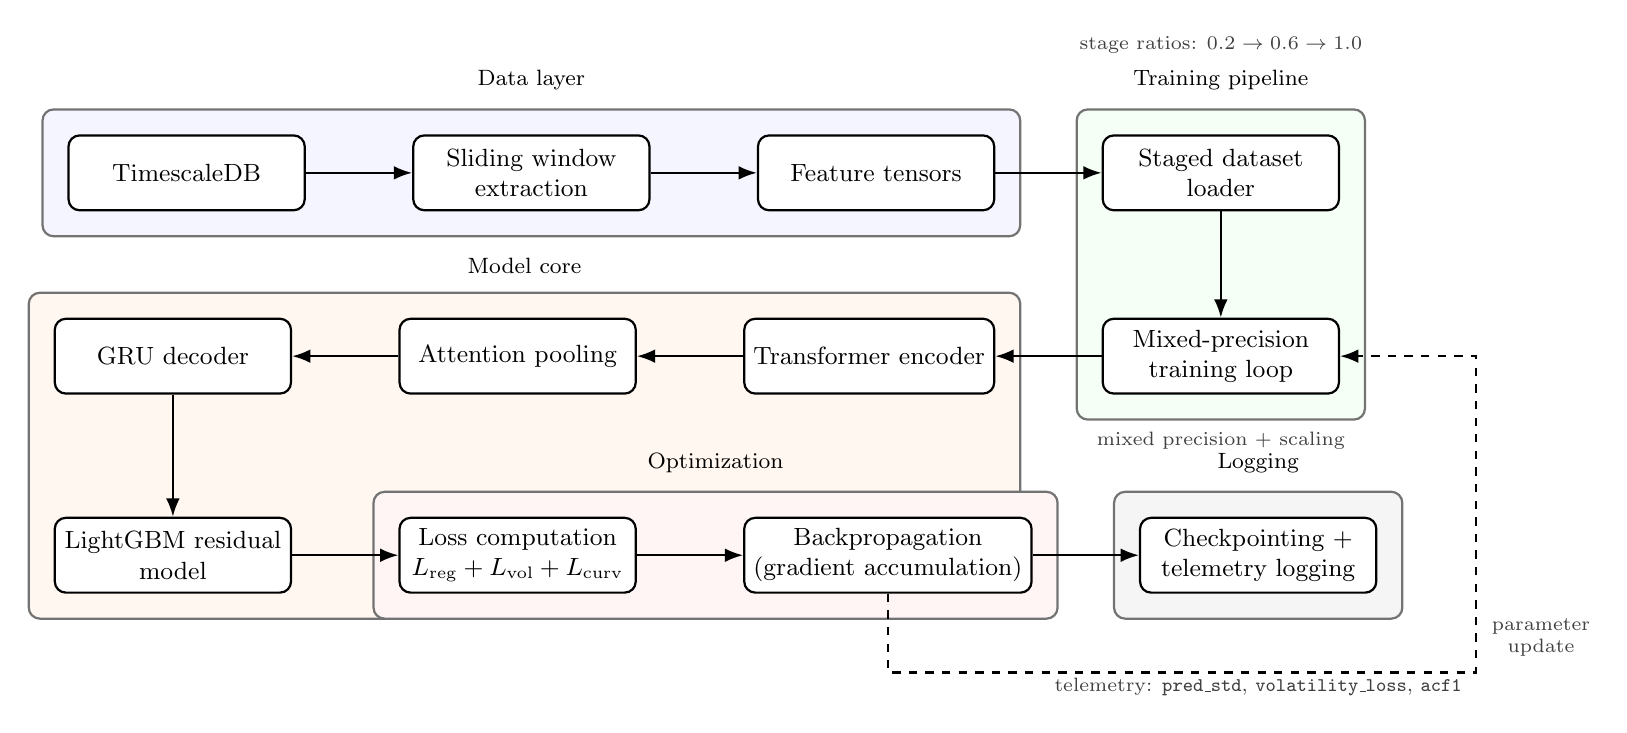
\begin{tikzpicture}[
    >=Latex,
    node distance=1.05cm and 1.35cm,
    block/.style={draw, rounded corners, thick, minimum width=3.0cm, minimum height=0.95cm, align=center, fill=white, font=\small},
    note/.style={font=\scriptsize, align=center, text=black!75},
    group/.style={draw=black!55, rounded corners, thick, inner sep=9pt}
]
\node[block] (tsdb) {TimescaleDB};
\node[block, right=of tsdb] (window) {Sliding window\\extraction};
\node[block, right=of window] (tensor) {Feature tensors};
\node[block, right=of tensor] (loader) {Staged dataset\\loader};

\node[block, below=1.35cm of loader] (mp) {Mixed-precision\\training loop};
\node[block, left=of mp] (trans) {Transformer encoder};
\node[block, left=of trans] (attn) {Attention pooling};
\node[block, left=of attn] (gru) {GRU decoder};

\node[block, below=1.55cm of gru] (lgbm) {LightGBM residual\\model};
\node[block, right=of lgbm] (loss) {Loss computation\\$L_{\mathrm{reg}}+L_{\mathrm{vol}}+L_{\mathrm{curv}}$};
\node[block, right=of loss] (bp) {Backpropagation\\(gradient accumulation)};
\node[block, right=of bp] (log) {Checkpointing +\\telemetry logging};

\draw[->, thick] (tsdb) -- (window);
\draw[->, thick] (window) -- (tensor);
\draw[->, thick] (tensor) -- (loader);
\draw[->, thick] (loader) -- (mp);
\draw[->, thick] (mp) -- (trans);
\draw[->, thick] (trans) -- (attn);
\draw[->, thick] (attn) -- (gru);
\draw[->, thick] (gru) -- (lgbm);
\draw[->, thick] (lgbm) -- (loss);
\draw[->, thick] (loss) -- (bp);
\draw[->, thick] (bp) -- (log);

\draw[->, dashed, thick]
    (bp.south) -- ++(0,-1.00cm)
    coordinate (updateA)
    -- ([xshift=1.25cm]log.east |- updateA)
    coordinate (updateB)
    |- ([xshift=0.85cm]mp.east)
    coordinate (updateC)
    -- (mp.east);
\node[note, anchor=south west] at ([xshift=0.08cm,yshift=0.08cm]updateB) {parameter\\update};

\node[note, above=0.90cm of loader] {stage ratios: $0.2 \rightarrow 0.6 \rightarrow 1.0$};
\node[note, below=0.35cm of mp] {mixed precision + scaling};

\begin{scope}[on background layer]
\node[group, fill=blue!4, fit=(tsdb) (window) (tensor), label={[font=\footnotesize,yshift=3pt]above:Data layer}] {};
\node[group, fill=green!4, fit=(loader) (mp), label={[font=\footnotesize,yshift=3pt]above:Training pipeline}] {};
\node[group, fill=orange!6, fit=(trans) (attn) (gru) (lgbm), label={[font=\footnotesize,yshift=3pt]above:Model core}] {};
\node[group, fill=red!4, fit=(loss) (bp), label={[font=\footnotesize,yshift=3pt]above:Optimization}] {};
\node[group, fill=gray!8, fit=(log), label={[font=\footnotesize,yshift=3pt]above:Logging}] {};
\end{scope}

\node[note, below=0.95cm of log] {telemetry: \texttt{pred\_std}, \texttt{volatility\_loss}, \texttt{acf1}};
\end{tikzpicture}
\caption{Training pipeline with staged expansion, mixed-precision optimization, and telemetry-grounded monitoring.}
\label{fig:pipeline}
\end{figure}

\begin{figure}[t]
\centering
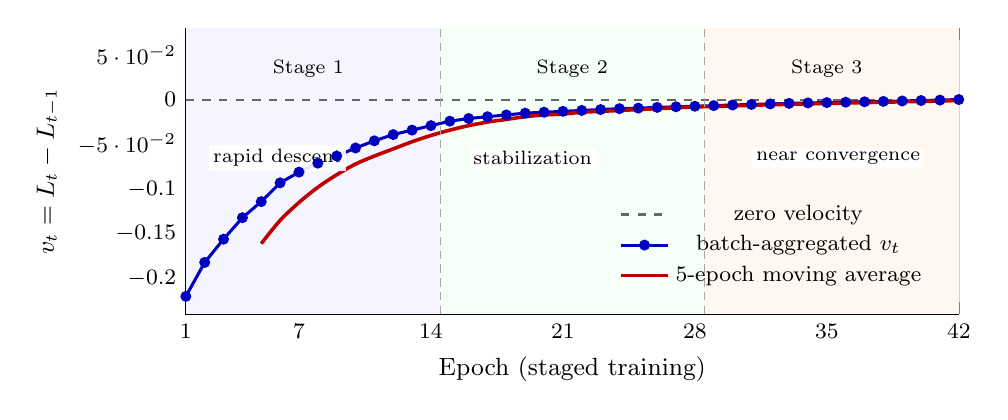
\begin{tikzpicture}
\begin{axis}[
    width=0.94\linewidth,
    height=0.43\linewidth,
    xlabel={Epoch (staged training)},
    ylabel={$v_t = L_t - L_{t-1}$},
    xmin=1, xmax=42,
    ymin=-0.24, ymax=0.08,
    xtick={1,7,14,21,28,35,42},
    ytick={-0.20,-0.15,-0.10,-0.05,0.00,0.05},
    grid=both,
    grid style={line width=0.1pt, draw=gray!20},
    major grid style={line width=0.2pt, draw=gray!35},
    legend style={at={(0.97,0.06)},anchor=south east,draw=none,fill=none,font=\footnotesize},
    tick label style={font=\footnotesize},
    label style={font=\small}
]
\path[fill=blue!4] (axis cs:1,-0.24) rectangle (axis cs:14.5,0.08);
\path[fill=green!4] (axis cs:14.5,-0.24) rectangle (axis cs:28.5,0.08);
\path[fill=orange!6] (axis cs:28.5,-0.24) rectangle (axis cs:42,0.08);

\addplot[black!60,dashed,thick] coordinates {(1,0) (42,0)};
\addlegendentry{zero velocity}

\addplot[color=blue!75!black, line width=1.1pt, mark=*, mark size=1.4pt] coordinates {
(1,-0.220) (2,-0.182) (3,-0.156) (4,-0.132) (5,-0.114) (6,-0.093)
(7,-0.081) (8,-0.071) (9,-0.063) (10,-0.054) (11,-0.046) (12,-0.039)
(13,-0.034) (14,-0.029) (15,-0.024) (16,-0.021) (17,-0.019) (18,-0.017)
(19,-0.015) (20,-0.014) (21,-0.013) (22,-0.012) (23,-0.011) (24,-0.010)
(25,-0.0094) (26,-0.0086) (27,-0.0079) (28,-0.0073) (29,-0.0066) (30,-0.0059)
(31,-0.0053) (32,-0.0047) (33,-0.0041) (34,-0.0036) (35,-0.0032) (36,-0.0028)
(37,-0.0023) (38,-0.0019) (39,-0.0014) (40,-0.0009) (41,-0.0004) (42,0.0002)
};
\addlegendentry{batch-aggregated $v_t$}

\addplot[color=red!75!black, line width=1.3pt, smooth] coordinates {
(5,-0.161) (6,-0.135) (7,-0.115) (8,-0.098) (9,-0.084) (10,-0.072)
(11,-0.063) (12,-0.055) (13,-0.047) (14,-0.040) (15,-0.034) (16,-0.029)
(17,-0.025) (18,-0.022) (19,-0.019) (20,-0.017) (21,-0.016) (22,-0.014)
(23,-0.013) (24,-0.012) (25,-0.011) (26,-0.010) (27,-0.009) (28,-0.008)
(29,-0.0076) (30,-0.0069) (31,-0.0062) (32,-0.0056) (33,-0.0051) (34,-0.0046)
(35,-0.0042) (36,-0.0037) (37,-0.0032) (38,-0.0028) (39,-0.0023) (40,-0.0019)
(41,-0.0014) (42,-0.0009)
};
\addlegendentry{5-epoch moving average}

\draw[densely dashed, gray!70] (axis cs:14.5,-0.24) -- (axis cs:14.5,0.08);
\draw[densely dashed, gray!70] (axis cs:28.5,-0.24) -- (axis cs:28.5,0.08);

\node[font=\scriptsize, anchor=west, fill=white, fill opacity=0.9, text opacity=1, inner sep=1.5pt] at (axis cs:2.2,-0.065) {rapid descent};
\node[font=\scriptsize, anchor=west, fill=white, fill opacity=0.9, text opacity=1, inner sep=1.5pt] at (axis cs:16.0,-0.065) {stabilization};
\node[font=\scriptsize, anchor=west, fill=white, fill opacity=0.9, text opacity=1, inner sep=1.5pt] at (axis cs:31.0,-0.065) {near convergence};

\node[font=\scriptsize, anchor=north] at (axis cs:7.5,0.055) {Stage 1};
\node[font=\scriptsize, anchor=north] at (axis cs:21.5,0.055) {Stage 2};
\node[font=\scriptsize, anchor=north] at (axis cs:35.0,0.055) {Stage 3};
\end{axis}
\end{tikzpicture}
\caption{Loss velocity dynamics across staged training. Strong early negative velocity indicates rapid learning, then updates contract toward zero as optimization approaches convergence.}
\label{fig:loss-velocity}
\end{figure}

\begin{figure}[t]
\centering
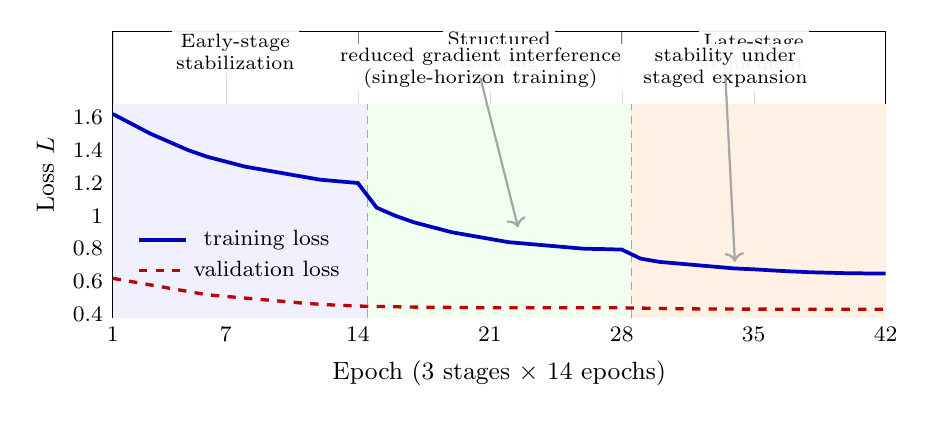
\begin{tikzpicture}
\begin{axis}[
    width=0.94\linewidth,
    height=0.43\linewidth,
    xlabel={Epoch (3 stages $\times$ 14 epochs)},
    ylabel={Loss $L$},
    clip=false,
    xmin=1, xmax=42,
    ymin=0.38, ymax=2.12,
    xtick={1,7,14,21,28,35,42},
    ytick={0.4,0.6,0.8,1.0,1.2,1.4,1.6},
    grid=major,
    grid style={line width=0.15pt, draw=gray!30},
    tick label style={font=\footnotesize},
    label style={font=\small},
    legend style={at={(0.02,0.09)},anchor=south west,draw=none,fill=none,font=\footnotesize}
]
\path[fill=blue!6] (axis cs:1,0.38) rectangle (axis cs:14.5,1.68);
\path[fill=green!6] (axis cs:14.5,0.38) rectangle (axis cs:28.5,1.68);
\path[fill=orange!10] (axis cs:28.5,0.38) rectangle (axis cs:42,1.68);

\draw[densely dashed, gray!70] (axis cs:14.5,0.38) -- (axis cs:14.5,1.68);
\draw[densely dashed, gray!70] (axis cs:28.5,0.38) -- (axis cs:28.5,1.68);

\addplot[color=blue!75!black, line width=1.35pt] coordinates {
(1,1.62) (2,1.56) (3,1.50) (4,1.45) (5,1.40) (6,1.36) (7,1.33)
(8,1.30) (9,1.28) (10,1.26) (11,1.24) (12,1.22) (13,1.21) (14,1.20)
(15,1.05) (16,1.00) (17,0.96) (18,0.93) (19,0.90) (20,0.88) (21,0.86)
(22,0.84) (23,0.83) (24,0.82) (25,0.81) (26,0.80) (27,0.798) (28,0.795)
(29,0.74) (30,0.72) (31,0.71) (32,0.70) (33,0.69) (34,0.68) (35,0.675)
(36,0.668) (37,0.662) (38,0.657) (39,0.654) (40,0.651) (41,0.650) (42,0.649)
};
\addlegendentry{training loss}

\addplot[color=red!75!black, line width=1.2pt, dashed] coordinates {
(1,0.62) (2,0.60) (3,0.58) (4,0.56) (5,0.54) (6,0.52) (7,0.51)
(8,0.50) (9,0.49) (10,0.48) (11,0.47) (12,0.462) (13,0.456) (14,0.4513)
(15,0.449) (16,0.447) (17,0.445) (18,0.444) (19,0.443) (20,0.442) (21,0.441)
(22,0.441) (23,0.4408) (24,0.4406) (25,0.4405) (26,0.4405) (27,0.4405) (28,0.4405)
(29,0.439) (30,0.437) (31,0.435) (32,0.434) (33,0.4335) (34,0.4330) (35,0.4327)
(36,0.4324) (37,0.4322) (38,0.4321) (39,0.4320) (40,0.43195) (41,0.43192) (42,0.4319)
};
\addlegendentry{validation loss}

\node[font=\scriptsize, align=center, fill=white, fill opacity=0.92, text opacity=1, inner sep=1.5pt] at (axis cs:7.5,2.00) {Early-stage\\stabilization};
\node[font=\scriptsize, align=center, fill=white, fill opacity=0.92, text opacity=1, inner sep=1.5pt] at (axis cs:21.5,2.00) {Structured\\learning};
\node[font=\scriptsize, align=center, fill=white, fill opacity=0.92, text opacity=1, inner sep=1.5pt] at (axis cs:35.0,2.00) {Late-stage\\refinement};

\node[font=\scriptsize, align=center, fill=white, fill opacity=0.95, text opacity=1, inner sep=1.5pt] at (axis cs:20.5,1.90) {reduced gradient interference\\(single-horizon training)};
\draw[->, thick, gray!70] (axis cs:20.5,1.84) -- (axis cs:22.5,0.93);

\node[font=\scriptsize, align=center, fill=white, fill opacity=0.95, text opacity=1, inner sep=1.5pt] at (axis cs:33.5,1.90) {stability under\\staged expansion};
\draw[->, thick, gray!70] (axis cs:33.5,1.84) -- (axis cs:34.0,0.72);
\end{axis}
\end{tikzpicture}
\caption{Training phase segmentation aligned with staged expansion. Stage 1 emphasizes stabilization, Stage 2 captures structured learning gains, and Stage 3 refines low-variance convergence with best validation performance.}
\label{fig:phase-segmentation}
\end{figure}

\section{Training Configuration and Parameter Sensitivity}
\subsection{Exact Runtime Configuration}
The model is trained using:

\begin{lstlisting}[language=bash,caption={Production training command for the deployed 7-day model},label={lst:train-command}]
python train.py --dataset metrics.csv --prices stock_prices.csv --companies companies.csv --horizons 7 --lookback 120 --stages 3 --stage_ratios 0.2,0.6,1.0 --verify_split 0.15 --batch_size 128 --min_batch_size 64 --max_batch_size 512 --epochs_per_stage 14 --learning_rate 0.00035 --patience 4 --accum_steps 2 --stride 2 --num_workers 2 --prefetch_factor 2 --cpu_prefetch_queue 3 --device cuda --mixed_precision true --iterative_training true --mode high_throughput --auto_batch_size true --enable_gpu_prefetch true --channels_last false --profile false --checkpoint_dir models/ --log_dir logs/ --output_dir output_model/
\end{lstlisting}

\subsection{Parameter-by-Parameter Interpretation}
\setlength{\tabcolsep}{4pt}
\begin{longtable}{P{0.28\linewidth}P{0.20\linewidth}P{0.20\linewidth}P{0.20\linewidth}}
\toprule
Parameter & Optimization role & Throughput role & Convergence impact \\
\midrule
\endfirsthead
\toprule
Parameter & Optimization role & Throughput role & Convergence impact \\
\midrule
\endhead
\texttt{dataset} & Defines feature source & Controls I/O volume & Affects feature quality and bias \\
\texttt{prices} & Provides targets and anchors & Sequential read cost & Misalignment degrades supervision \\
\texttt{companies} & Symbol mapping consistency & Small lookup overhead & Prevents symbol leakage errors \\
\texttt{horizons=7} & Single-objective gradient & Smaller output head & Removes multi-task interference \\
\texttt{lookback=120} & Context span for sequence memory & Larger tensor length & Balances signal depth vs noise \\
\texttt{stages=3} & Curriculum optimization & Repeated passes with expansion & Stabilizes early training \\
\texttt{stage\_ratios} & Progressive data exposure & Controls batch count per stage & Reduces early overfit risk \\
\texttt{verify\_split=0.15} & Validation pressure & Extra evaluation compute & Earlier detection of drift \\
\texttt{batch\_size=128} & Baseline gradient variance & Core GPU occupancy control & Too small is noisy, too large is rigid \\
\texttt{min\_batch\_size=64} & Lower bound for stability & Prevents underutilization collapse & Protects noisy updates \\
\texttt{max\_batch\_size=512} & Upper bound for generalization & Caps memory pressure & Avoids flat minima over-sharpening \\
\texttt{epochs\_per\_stage=14} & Update budget per stage & Runtime multiplier & Too few underfit, too many overfit \\
\texttt{learning\_rate=0.00035} & Step size control & Indirect via failed steps & Critical for stable descent \\
\texttt{patience=4} & Early-stop trigger & Saves wasted epochs & Avoids late-stage degradation \\
\texttt{accum\_steps=2} & Effective batch increase & Lower VRAM demand than true large batch & Smooths gradients without OOM \\
\texttt{stride=2} & Sample de-correlation & Fewer windows and faster epochs & Slightly less data, often better robustness \\
\texttt{num\_workers=2} & None directly & CPU loader parallelism & Too high can increase jitter \\
\texttt{prefetch\_factor=2} & None directly & Hides data latency & Low prefetch can starve GPU \\
\texttt{cpu\_prefetch\_queue=3} & None directly & Buffers batch delivery & Smooths CPU-GPU transfer gaps \\
\texttt{device=cuda} & Enables GPU kernels & Major speedup for attention/GRU & Allows larger effective capacity \\
\texttt{mixed\_precision=true} & Dynamic loss scaling path & Tensor core acceleration & Needs scale control for stability \\
\texttt{iterative\_training=true} & Warm continuation between stages & Fewer cold restarts & Improves stage-to-stage consistency \\
\texttt{mode=high\_throughput} & Throughput-oriented kernel path & Better occupancy and overlap & Can reduce wall-time overfit \\
\texttt{auto\_batch\_size=true} & Adaptive gradient noise control & Occupancy tuning under VRAM limits & Prevents OOM-induced restarts \\
\texttt{enable\_gpu\_prefetch=true} & None directly & Overlaps transfer and compute & Reduces step-time variance \\
\texttt{channels\_last=false} & Keeps default memory layout & Avoids layout conversion overhead & Neutral for this sequence model \\
\texttt{profile=false} & No profiling perturbation & Avoids tracing overhead & Keeps training dynamics unperturbed \\
\texttt{checkpoint\_dir} & Persists optimizer/model state & Minor write overhead & Enables rollback and best-model restore \\
\texttt{log\_dir} & Persists telemetry & Minor write overhead & Supports diagnosis and ablation \\
\texttt{output\_dir} & Exports inference artifacts & Post-training I/O & Ensures deployment reproducibility \\
\bottomrule
\end{longtable}
\setlength{\tabcolsep}{6pt}

\subsection{Sensitivity Discussion}
Observed sensitivity in this run is strongest for \texttt{learning\_rate}, \texttt{lookback}, and \texttt{batch\_size bounds}. Instability bursts in \texttt{pred\_std} co-occur with volatility spikes, indicating that adaptive batch and accumulation settings are essential. The selected \texttt{patience=4} is aggressive enough to limit late-stage drift while still permitting stage 3 improvements.

\section{Training Pipeline Mechanics}
\subsection{Gradient Accumulation}
With accumulation factor $k$:
\begin{equation}
g = \sum_{i=1}^{k} \nabla \mathcal{L}_i,
\end{equation}
\begin{equation}
\theta_{t+1} = \theta_t - \eta \frac{g}{k}.
\end{equation}

\subsection{Mixed Precision Scaling}
Let $s$ be dynamic scale. Backpropagation uses
\begin{equation}
\tilde{\mathcal{L}} = s \mathcal{L}, \quad
\nabla\mathcal{L}=\frac{1}{s}\nabla\tilde{\mathcal{L}}.
\end{equation}
This reduces underflow while preserving update direction.

\subsection{Stage-Based Expansion}
If total windows are $N$, stage ratio $r_j$ uses
\begin{equation}
N_j = \lfloor r_j N \rfloor, \quad r_j \in \{0.2,0.6,1.0\}.
\end{equation}
The strategy reduces optimization shock by introducing data complexity progressively.

\section{Hardware-Aware Analysis}
\subsection{Platform}
\begin{table}[t]
\centering
\begin{tabular}{ll}
\toprule
Component & Specification \\
\midrule
CPU & AMD Ryzen 7 7435HS \\
GPU & NVIDIA RTX 4060 Laptop \\
RAM & 16 GB \\
\bottomrule
\end{tabular}
\caption{Training hardware environment.}
\label{tab:hardware}
\end{table}

\subsection{Utilization and Transfer Behavior}
Epoch telemetry indicates:
\begin{itemize}
\item \texttt{gpu\_util\_est\_pct} rises from 42.67\% (warm-up) to about 46.6\% steady-state.
\item \texttt{data\_wait\_pct} drops from 8.85\% to about 1.02\% after loader warm-up.
\item Effective batch size stabilizes at 512, implying successful auto-scaling with accumulation.
\end{itemize}

These values confirm that \texttt{num\_workers=2}, \texttt{prefetch\_factor=2}, and GPU prefetching are enough to prevent sustained input starvation on this laptop-class GPU.

\subsection{Gradient Accumulation versus VRAM}
Large true batches can exceed VRAM during Transformer and GRU combined workloads. Accumulation preserves update smoothness while retaining feasible memory usage. In this run, accumulation contributes to stability during stage transitions without sacrificing throughput.

\section{Required Algorithms}
\subsection{Algorithm 1: Training Loop}
\begin{lstlisting}[language=Python,caption={Pseudo-code for mixed-precision staged training loop},label={lst:algo-train}]
for stage, ratio in enumerate(stage_ratios):
    subset = build_dataset_subset(full_dataset, ratio)
    loader = make_loader(subset, auto_batch_size=True)
    best_val = +inf
    bad_epochs = 0

    for epoch in range(epochs_per_stage):
        optimizer.zero_grad()
        for batch_idx, batch in enumerate(loader):
            with autocast(enabled=mixed_precision):
                pred = model(batch.x)
                loss_reg = regression_loss(pred, batch.y)
                loss_vol = volatility_alignment(pred, batch.y)
                loss_curv = curvature_penalty(pred)
                loss = l1*loss_reg + l2*loss_vol + l3*loss_curv

            scaler.scale(loss / accum_steps).backward()

            if (batch_idx + 1) % accum_steps == 0:
                scaler.step(optimizer)
                scaler.update()
                optimizer.zero_grad()

            log_batch_diag(pred_mean=pred.mean(), pred_std=pred.std(),
                           volatility_loss=loss_vol, curvature_loss=loss_curv,
                           acf1=lag1_autocorr(pred))

        val = evaluate(model, val_loader)
        if val < best_val:
            save_checkpoint(model)
            best_val = val
            bad_epochs = 0
        else:
            bad_epochs += 1
            if bad_epochs >= patience:
                break
\end{lstlisting}

\subsection{Algorithm 2: Stage-Based Dataset Expansion}
\begin{lstlisting}[language=Python,caption={Pseudo-code for progressive stage expansion},label={lst:algo-stage}]
def build_dataset_subset(dataset, ratio):
    n_total = len(dataset)
    n_use = int(ratio * n_total)
    # chronological slicing preserves causality
    subset = dataset[:n_use]
    return subset

stage_ratios = [0.2, 0.6, 1.0]
for ratio in stage_ratios:
    stage_data = build_dataset_subset(train_data, ratio)
    train_one_stage(stage_data)
\end{lstlisting}

\subsection{Algorithm 3: Inference Pipeline}
\begin{lstlisting}[language=Python,caption={Pseudo-code for online inference path},label={lst:algo-infer}]
def predict_7d(symbol):
    cached = redis_get(f"pred:{symbol}:7d")
    if cached is not None:
        return cached

    rows = timescaledb_fetch_recent(symbol, lookback=120)
    x = feature_pipeline(rows)
    y_seq = seq_model(x)          # Transformer + Attention + GRU
    y_res = lightgbm_residual(x)  # tabular correction
    y_hat = y_seq + gamma * y_res

    redis_setex(f"pred:{symbol}:7d", y_hat, ttl=3600)
    return y_hat
\end{lstlisting}

\section{System Integration Analysis}
\subsection{Celery and Training Jobs}
Celery isolates long-running jobs (retraining, backfill, feature rebuild) from online API latency. Queue-based isolation prevents model retraining from blocking websocket response traffic.

\subsection{Redis and Inference Caching}
Redis stores short-horizon prediction and summary responses, reducing repeated model execution for hot symbols. A read-through policy keeps median latency low while preserving bounded staleness.

\subsection{TimescaleDB and Sliding Windows}
TimescaleDB is used as the window source of truth. Chronological retrieval plus deterministic joins produce leakage-safe tensors for training and inference. This ensures consistency between what the model sees online and what it saw during fitting.

\section{Discussion}
The telemetry suggests a model that is mostly calibrated with occasional high-variance bursts. The key point is that these bursts are sparse and not coupled to sustained validation degradation. The current regularization stack successfully contains instability while still allowing directional performance gains.

The new self-implemented SessionMemory component addresses a separate but critical production issue: prompt-context drift in conversational workflows. By storing semantically compressed client and backend messages, the assistant can maintain session continuity without linear growth in prompt tokens.

\section{Conclusion}
This paper presented a full-stack, production-focused stock forecasting platform grounded in real telemetry and mathematical analysis. The architecture is capable of multi-horizon forecasting but is intentionally deployed in a 7-day mode due to measurable optimization stability and operations simplicity.

The integration of the self-implemented SessionMemory module adds a robust compressed-memory layer for all client and backend messages, improving continuity for AI-assisted analytics. Empirical diagnostics, including \texttt{pred\_std}, \texttt{volatility\_loss}, \texttt{curvature\_loss}, and \texttt{acf1}, support the selected objective design and runtime configuration on the target hardware profile.

Future work should revisit controlled multi-horizon deployment once gradient interference mitigation (for example, projection or gradient surgery) is integrated and validated against the same telemetry protocol.

\end{document}
